\chapter{Thiết kế hệ thống truyền động}
\section{Tính bộ phận công tác}
\subsection{Tính bước của trục vít tải}
\begin{itemize}
    \item Ta chọn vật liệu là Inox 304 vì nó có độ bền cao, khả năng chống ăn mòn tốt phù hợp với môi trường làm việc của máy ép bùn.
    \item Ta sử dụng vít tải quay chậm để vận chuyển vật liệu theo phương nằm ngang. 
    \item Khi trục vít quay thì vật liệu được nâng lên và cả khối vật liệu bị nghiêng đi một góc $\varphi $ như hình dưới, tại đó trọng lượng của vật liệu sẽ cân bằng với lực ma sát của vật liệu với thành máy.
\end{itemize}
\begin{figure}[H]
    \centering
    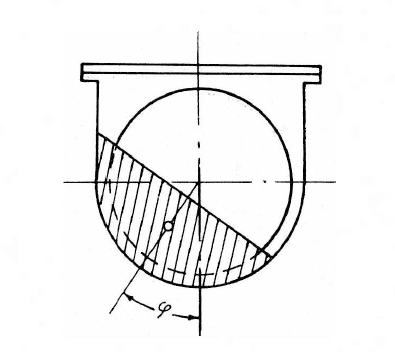
\includegraphics[width=0.5\textwidth]{pictures/vittai1.png}
    \caption{Sự phân bố của vật liệu khi trục vít tải quay}
\end{figure}

\begin{itemize}
    \item Bước của trục vít (hay khoảng cách giữa các cánh vít) đối với vật liệu dạng bột hoặc hạt nhỏ được xác định là:
    \[
        S = (0.7 \div 1)D = 1 \cdot 225 = 225 (mm) 
    \]
\end{itemize}

\subsection{Diện tích tiết diện ngang do vật liệu chiếm trong thành máy}
\[
    F = \frac{\pi\cdot D^2}{4}\mu \cdot K = \frac{\pi\cdot 0.225^2}{4}\cdot 0.35\cdot 1 = 0.0139 (m^2)
\]
Trong đó: 
\begin{itemize}
    \item D = 225 mm, là đường kính của vít tải
    \item $\mu$ là hệ số chứa vật liệu trong thành máy. Với vật liệu dạng bột ta chọn $\mu = 0.35$
    \item K là hệ số chỉ sự giảm tiết diện do góc nghiêng đặt vít tải. Với góc nghiêng bằng $0^{\circ}$ ta chọn $K = 1$
\end{itemize}
\subsection{Vận tốc chuyển vật liệu dọc theo trục vít}
\[
    v = \frac{S\cdot n_{ct}}{60} = \frac{0.225\cdot 118.85}{60} = 0.4434 (m/s)
\]
Trong đó: 
\begin{itemize}
    \item $S = 225 mm$: bước của vít tải
    \item $n_{ct} = 118.85$ vòng/phút: số vòng quay của trục vít tải
\end{itemize}
\subsection{Xác định năng xuất máy}
\[
    Q = 3600F\cdot v\cdot \rho = 3600\cdot 0.0139\cdot 0.4434\cdot 1000 = 22187.74 (kg/h)
\]
Trong đó:
\begin{itemize}
    \item $F = 13916.27 mm^2$: diện tích ngang do vật liệu chiếm trong thành máy
    \item $v = 0.4434$ m/s: vận tốc chuyển vật liệu dọc theo trục vít
    \item $\rho = 1000$ kg/m$^3$: khối lượng riêng của bùn
\end{itemize}
\section{Thùng cấp liệu}
\begin{itemize}
    \item Vật liệu: Inox 304
    \item Kích thước: 170x170x75 mm
    \item Tùy theo như cầu sử dụng mà có thể thay đổi kích thước của thùng cấp liệu cho phù hợp với yêu cầu của máy.
\end{itemize}
\begin{figure}[H]
    \centering
    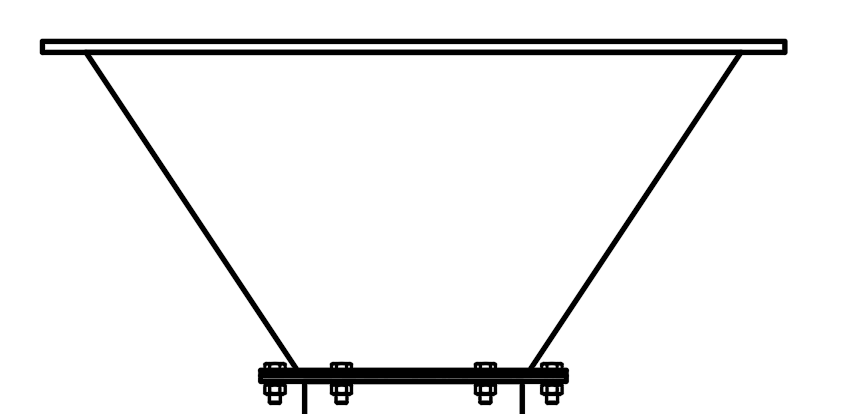
\includegraphics[width=0.5\textwidth]{pictures/thungcap.png}
    \caption{Thùng cấp liệu}
\end{figure}

\section{Vít tải}
\begin{itemize}
    \item Vật liệu: Inox 304
    \item Đường kính: 225 mm
    \item Tùy theo như cầu sử dụng mà có thể thay đổi kích thước của vít tải cho phù hợp với yêu cầu của máy.
\end{itemize}
\begin{figure}[H]
    \centering
    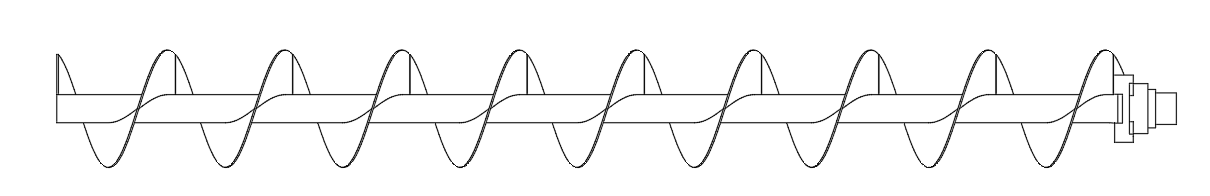
\includegraphics[width=1\textwidth]{pictures/vit.png}
    \caption{Vít tải}
\end{figure}

\section{Thân máy hình máng}
\begin{itemize}
    \item Vật liệu: Inox 304
    \item Đường kính: 300 mm
    \item Thân máy được nối với thùng cấp liệu bằng bulong và đai ốc.
    \item Thân máy có chỗ xả liệu để xả bùn ra ngoài.
\end{itemize}
\begin{figure}[H]
    \centering
    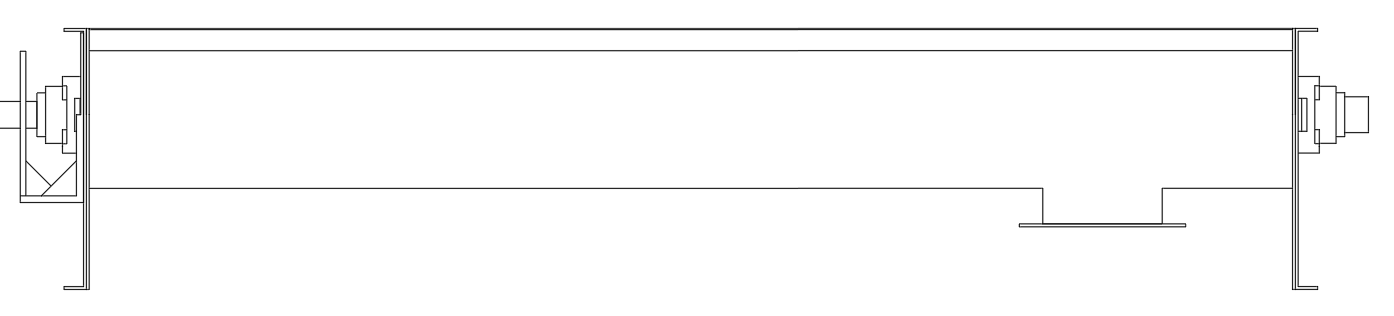
\includegraphics[width=1\textwidth]{pictures/than.png}
    \caption{Thân máy hình máng}
\end{figure}

\section{Bệ đỡ động cơ và hộp giảm tốc}
\begin{itemize}
    \item Vật liệu: Thép.
    \item Cố định các đơn vị lắp lên bệ đỡ bằng bulong và đai ốc.
    \item Có thể sử dụng phương pháp hàn để cố định các bệ đỡ.
\end{itemize}
\begin{figure}[H]
    \centering
    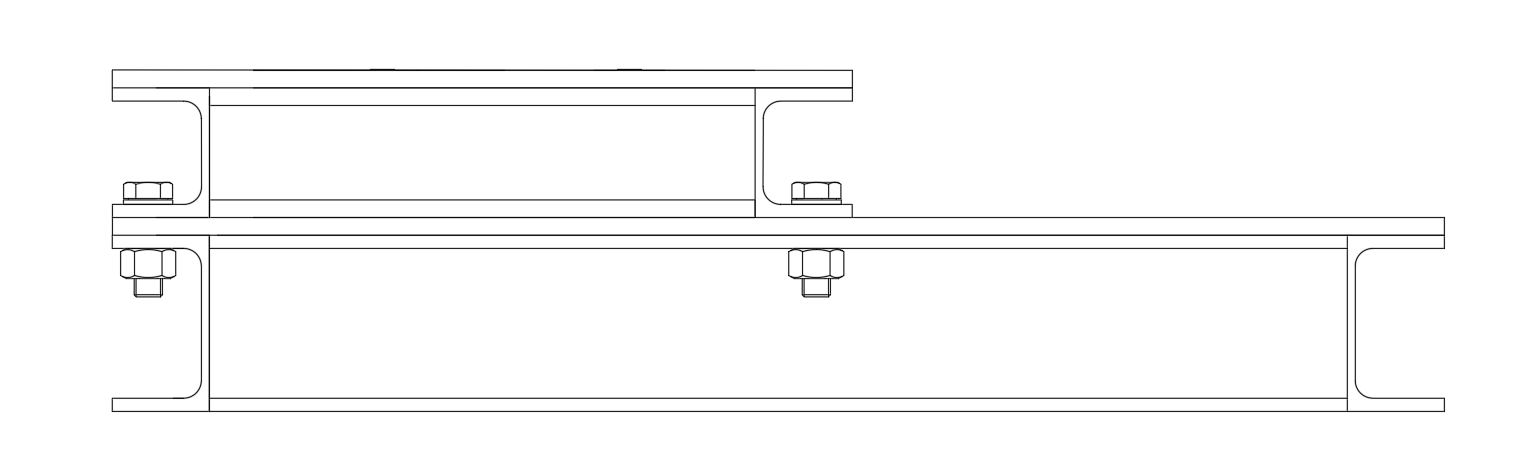
\includegraphics[width=1\textwidth]{pictures/be.png}
    \caption{Bệ đỡ động cơ và hộp giảm tốc}
\end{figure}

\section{Bộ phận căng đai}
\begin{itemize}
    \item Chế tạo từ các tấm thép khi sản xuất đơn chiếc.
    \item Sử dụng gang xám khi sản xuất hàng loạt.
    \item Bộ phận căng đai được lắp trên bệ đỡ động cơ và hộp giảm tốc.
    \item Căng đai bằng phương pháp dịch chuyển động cơ tịnh tiến.
    \item Cố định với bệ đỡ và động cơ bằng bulong và đai ốc.
\end{itemize}
\begin{figure}[H]
    \centering
    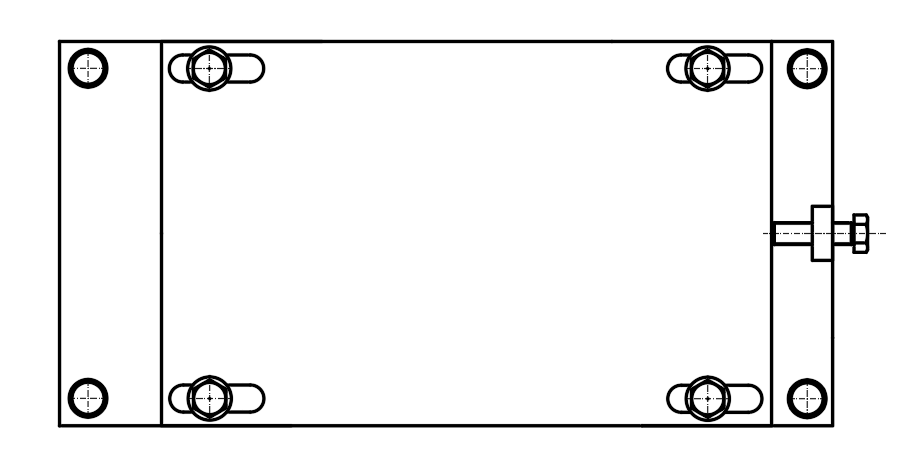
\includegraphics[width=0.7\textwidth]{pictures/cangdai.png}
    \caption{Bộ phận căng đai}
\end{figure}

\section{Gối đỡ vòng bi}
\begin{itemize}
    \item Mã sản phẩm: FY 45 FM
    \item Nhà sản xuất: SKF
    \item Đường kính trục: 45 mm
    \item Kiểu gối đỡ: Mặt bích vuông 4 lỗ
    \item Vật liệu vỏ: Gang đúc
    \item Loại vòng bi: Vòng bi cầu (ball bearing)
    \item Tải trọng động: 33,2 kN
    \item Tải trọng tĩnh: 21,6 kN
    \item Tốc độ tối đa: 4.300 vòng/phút
\end{itemize}
\begin{figure}[H]
    \centering
    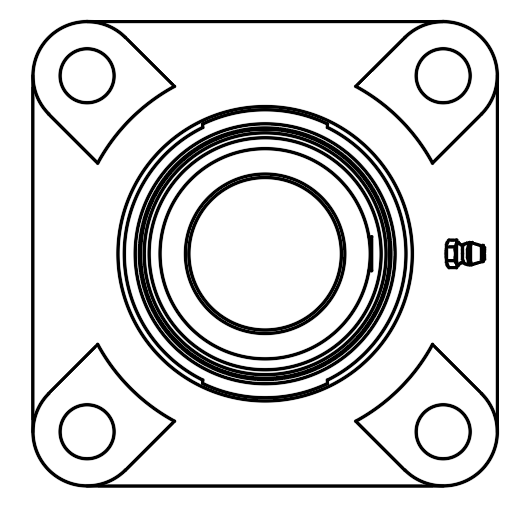
\includegraphics[width=0.4\textwidth]{pictures/goi.png}
    \caption{Gối đỡ vòng bi}
\end{figure}